% Numeración del capítulo: 3.
\setcounter{chapter}{2}

\chapter{\textit{Pipeline} de preprocesamiento}\label{chap:preprocesamiento}

El presente capítulo describe el segundo componente técnico del sistema: el \textit{pipeline} de preprocesamiento que transforma una imagen de página digitalizada en una lista de líneas de texto listas para su procesamiento por el modelo de reconocimiento que el capítulo~\ref{chap:modelo} desarrolla. El capítulo se organiza en cinco secciones. La sección~\ref{sec:analisis-imagen} describe el análisis preliminar de la imagen y la configuración automática del \textit{pipeline} a partir de las métricas que el análisis produce. La sección~\ref{sec:binarizacion} detalla la binarización y el criterio de selección automática entre los dos métodos disponibles. La sección~\ref{sec:correccion-inclinacion} expone la corrección de inclinación a tres niveles: global de la página, residual por bloque y por línea. La sección~\ref{sec:deteccion-segmentacion} explica la detección de bloques de texto y la segmentación de líneas dentro de cada bloque. La sección~\ref{sec:normalizacion-lineas} describe la normalización final que produce las líneas con la altura fija que el modelo exige.

% -----------------------------------------------------------------------------
\section{Análisis de imagen y configuración automática}
\label{sec:analisis-imagen}

Las imágenes que el sistema recibe como entrada presentan una diversidad amplia de condiciones visuales. Una digitalización profesional de un libro tiene fondo claro y uniforme, iluminación homogénea, contraste alto y trazos nítidos. Una fotografía tomada con un teléfono móvil puede presentar gradientes de iluminación, sombras locales, ruido del sensor y baja resolución. Un documento antiguo digitalizado puede tener fondo amarillento, tinta desvanecida, manchas y desalineación. Cada condición exige parámetros distintos en las etapas posteriores del \textit{pipeline}.

Una primera opción consistiría en exponer los parámetros del \textit{pipeline} al usuario y dejar que los ajustara para cada imagen. El trabajo descarta la opción por dos razones. Primero, el usuario objetivo del sistema es un investigador o archivista que carece de formación en procesamiento de imágenes. Segundo, el ajuste manual para cada documento es incompatible con el procesamiento por lotes que requiere la digitalización masiva del acervo. El \textit{pipeline} adopta en su lugar una estrategia de configuración automática, que utiliza el cálculo de ciertas métricas de la imagen para definir los parámetros de la configuración.

El análisis calcula cinco métricas sobre la imagen en escala de grises. La primera es el contraste, que el sistema define como la diferencia entre los percentiles~95 y~5 de los valores de gris. La elección de percentiles, en lugar del rango máximo y mínimo, descarta píxeles anómalos que producen los reflejos puntuales o el ruido aislado. La segunda es la luminancia media. La tercera es la polaridad del fondo, que el sistema define a partir de la media de las esquinas de la imagen, con exclusión de franjas laterales que podrían contener bandas oscuras de encuadernación. Si la media de las esquinas resulta inferior a~127, el sistema considera oscuro el fondo y la binarización posterior invierte. La cuarta y la quinta son la altura estimada del texto y el número estimado de líneas, que el análisis calcula a partir de la proyección horizontal de una binarización preliminar mediante Otsu~\cite{otsu1979threshold}, con identificación de picos por la función \textit{find\_peaks} sobre la proyección que un filtro uniforme suaviza. La figura~\ref{fig:metricas-ejemplo} ilustra los valores que el análisis produce sobre una página real del archivo, junto con las decisiones de configuración que las cinco métricas inducen.

\begin{figure}[!htbp]
	\centering
	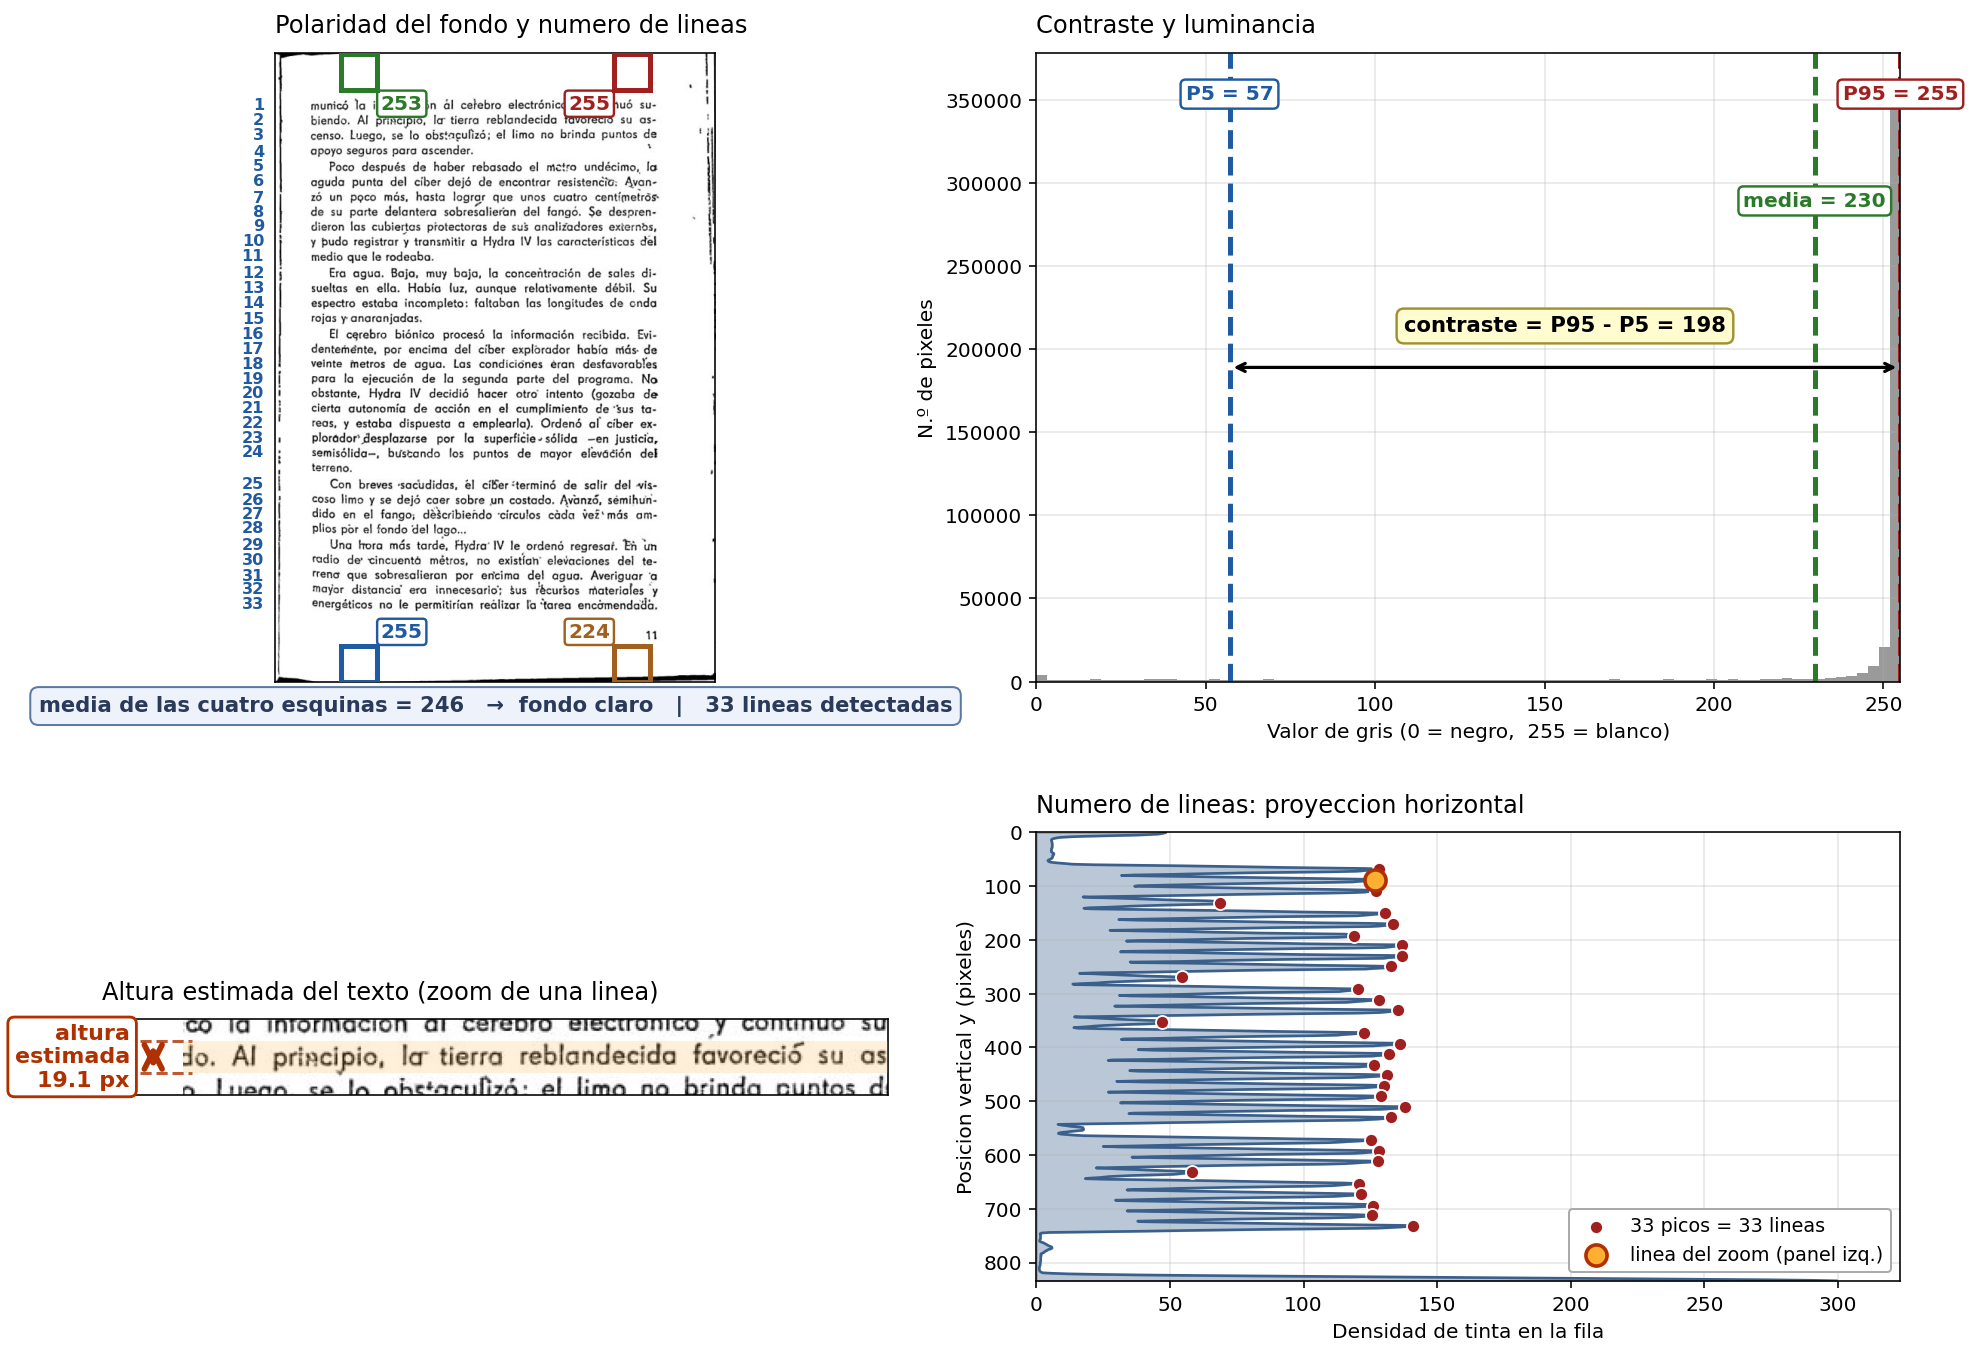
\includegraphics[width=\textwidth]{Graphics/analisis_metricas.png}
	\caption{Visualización de las cinco métricas que el análisis preliminar produce sobre una página real del archivo. El panel superior izquierdo muestra la imagen original con las cuatro esquinas que el sistema muestrea para decidir la polaridad del fondo y con la numeración de las líneas detectadas. El panel superior derecho muestra el histograma de intensidades con los percentiles~5 y~95, la luminancia media y el contraste como diferencia entre ambos percentiles. El panel inferior izquierdo presenta el zoom de una línea concreta con la cota de la altura estimada del texto. El panel inferior derecho muestra la proyección horizontal de la tinta, con cada pico que corresponde a una línea; el pico naranja resalta la línea que el panel del zoom amplía.}
	\label{fig:metricas-ejemplo}
\end{figure}

Las cinco métricas alimentan una función de configuración automática que devuelve los parámetros del \textit{pipeline}. Las decisiones de la configuración son las siguientes:

\begin{enumerate}[leftmargin=*,labelsep=0.5em]
	\item \textbf{Ecualización adaptativa del histograma.} Si el contraste cae por debajo de~60, el sistema activa la ecualización adaptativa del histograma con limitación de contraste, que la literatura denomina CLAHE~\cite{zuiderveld1994clahe} por sus siglas inglesas, junto con un filtro bilateral que reduce el ruido sin difuminar los bordes.
	\item \textbf{Ventana de Sauvola.} El sistema dimensiona la ventana del método de Sauvola~\cite{sauvola2000binarization} en función de la altura estimada del texto, garantizando que la vecindad de análisis cubra al menos una vez y media la altura de un carácter.
	\item \textbf{Parámetro $k$ de Sauvola.} El sistema ajusta el parámetro de sensibilidad de Sauvola en tres tramos según el contraste, con valores entre~0,10 y~0,25.
	\item \textbf{Inversión binaria.} El sistema activa la inversión cuando el fondo resulta oscuro, según la polaridad que la tercera métrica determina.
	\item \textbf{Dilatación vertical y altura mínima por línea.} El sistema calibra la dilatación vertical que la detección de líneas emplea, y la altura mínima que admite por línea, sobre la altura estimada del texto.
\end{enumerate}

El resultado del análisis es una configuración del \textit{pipeline} adaptable a las particularidades de cada imagen sin intervención del usuario. El \textit{pipeline} aplica la configuración en las etapas siguientes, que la presente sección describe a continuación.

% -----------------------------------------------------------------------------
\section{Binarización}
\label{sec:binarizacion}

La binarización es la operación que asigna a cada píxel el valor 0 si pertenece al fondo o el valor 1 si pertenece a tinta. La operación es necesaria por dos razones. La primera es que las etapas posteriores del \textit{pipeline}, como la detección de bloques y la segmentación de líneas, operan sobre proyecciones y componentes conexas existentes solo en imágenes binarias. La segunda es que la binarización elimina la variabilidad cromática y tonal de la imagen original, reduciendo el espacio de variación que el modelo debe aprender a tolerar.

El \textit{pipeline} dispone de dos métodos de binarización con propiedades complementarias. El primer método es la binarización global de Otsu~\cite{otsu1979threshold}, que calcula un único umbral para toda la imagen a partir del histograma bimodal de los valores de gris. El método escoge el umbral como el valor que maximiza la varianza entre las dos clases, una correspondiente al fondo y la otra a la tinta. Otsu produce trazos con el grosor natural del raster original, lo que resulta deseable cuando el fondo es uniforme y la separación entre tinta y papel es clara. El segundo método es la binarización adaptativa de Sauvola~\cite{sauvola2000binarization}, que calcula un umbral local para cada píxel a partir de la media~$\mu$ y la desviación típica~$\sigma$ de los valores de gris en una vecindad de tamaño fijo. El umbral local resulta de la fórmula:

\begin{equation}
	T(x, y) = \mu(x, y)\left[1 + k \left(\frac{\sigma(x, y)}{R} - 1\right)\right],
	\label{eq:sauvola}
\end{equation}

donde $k$ es un parámetro de sensibilidad y~$R$ es el rango dinámico esperado de la desviación típica. Sauvola compensa variaciones de iluminación que un umbral global no podría capturar, a costa de engrosar los trazos en aproximadamente el 15--25\,\% respecto al grosor natural.

La selección automática del método se basa en una medida de uniformidad del fondo. El \textit{pipeline} estima la desviación típica de los píxeles de fondo de la imagen tras una binarización preliminar y compara el valor con un umbral empírico que el sistema fija en~12. Por debajo del umbral, el sistema considera uniforme el fondo y aplica Otsu. Por encima, aplica Sauvola. El trabajo calibró el umbral sobre un conjunto pequeño de imágenes de prueba que abarcan tanto digitalizaciones limpias de libros como fotografías con iluminación irregular.

Tras la binarización, el \textit{pipeline} aplica una secuencia de operaciones de limpieza. La apertura morfológica~\cite{soille2003morphology} con un elemento estructurante cuadrado de dos píxeles elimina el moteado fino. El filtrado de componentes conexos descarta cualquier componente con área inferior a cuatro píxeles, valor por debajo del tamaño de los puntos sobre las íes y de los acentos en cualquier tipografía razonable, sin afectar al texto legítimo. La salida es una imagen binaria limpia, lista para las etapas siguientes.

% -----------------------------------------------------------------------------
\section{Corrección de inclinación y curvatura}
\label{sec:correccion-inclinacion}

Las imágenes de documentos digitalizados rara vez presentan las líneas de texto perfectamente horizontales. Una digitalización hecha a mano puede introducir una rotación leve de hasta tres o cuatro grados. Una fotografía de un teléfono móvil añade además distorsión perspectiva que curva el \textit{baseline} de las líneas. Un libro entero digitalizado presenta inclinaciones distintas en cada página del pliego, y a veces incluso en cada columna. El \textit{pipeline} corrige la inclinación a tres niveles sucesivos, cada uno con un alcance espacial diferente.

El primer nivel es la corrección global de la página. La operación, que la literatura denomina \textit{deskew}, busca el ángulo de rotación que devuelve las líneas de texto a la horizontalidad sobre la imagen completa. El método descansa sobre la transformada de Hough~\cite{duda1972hough}, en su variante probabilística. Hough no opera directamente sobre la imagen binaria, donde cada glifo es un cúmulo denso de píxeles que generaría falsas líneas, sino sobre una imagen de bordes que el operador de Canny~\cite{canny1986edge} produce en un paso previo. Canny suaviza la imagen con un filtro gaussiano, calcula los gradientes mediante un operador tipo Sobel, suprime los píxeles que no son máximos locales del gradiente y aplica una umbralización por histéresis con dos umbrales, en este caso~50 y~150. El resultado es una imagen donde solo los píxeles de contorno están activos, lo que reduce cada glifo a su silueta y deja una nube de puntos que cae aproximadamente sobre los \textit{baselines} de cada línea. Hough sobre esos contornos identifica segmentos rectos, cada uno con un ángulo, que el sistema pondera por el cuadrado de su longitud. La ponderación cuadrática hace que los segmentos largos, que corresponden a los \textit{baselines} de líneas completas, dominen sobre los segmentos cortos que generan los trazos oblicuos de letras individuales. El ángulo de corrección es la mediana ponderada de la distribución, que el sistema descarta cuando el rango intercuartílico supera cuatro grados, lo que indicaría una distribución multimodal incompatible con una única inclinación global.

El segundo nivel es la corrección residual por bloque, que el \textit{pipeline} aplica después de la corrección global. La operación ataca el caso de páginas con dos columnas o pliegos abiertos donde cada bloque presenta su propia inclinación residual respecto a la página. La estimación del ángulo opera con un método análogo al del nivel global, que el sistema restringe al recorte del bloque y con un rango angular más conservador.

El tercer nivel es la corrección de curvatura por línea, que la literatura denomina \textit{straightening}~\cite{zhang2002straightening}. La operación corrige las distorsiones que sobreviven a las correcciones lineales anteriores, típicamente el sangrado central que aparece en la digitalización de páginas cerca del lomo del libro y la curvatura que generan las fotografías con perspectiva. El método estima el \textit{baseline} de la línea como una curva polinomial de grado dos. Para construir la estimación, el método divide la línea en rebanadas verticales y calcula el centroide vertical de la tinta dentro de cada rebanada. Un ajuste por mínimos cuadrados aproxima el conjunto de pares (centro horizontal de la rebanada, centroide vertical de la tinta) a un polinomio de grado dos. El método acepta el ajuste solo si el coeficiente de determinación supera~0,72 y si el desplazamiento implícito no excede el 20\,\% de la altura de la línea. La aceptación condicional protege contra correcciones espurias en líneas demasiado cortas o con tinta dispersa, donde el ajuste polinomial podría sobreajustarse al ruido.

El conjunto de las tres correcciones cubre el rango de distorsiones que el sistema puede encontrar en la práctica, desde la rotación global uniforme hasta la curvatura local del \textit{baseline}.

% -----------------------------------------------------------------------------
\section{Detección y segmentación de bloques y líneas de texto}
\label{sec:deteccion-segmentacion}

El modelo de reconocimiento opera sobre líneas de texto individuales. El \textit{pipeline} debe, por tanto, identificar dónde empieza y termina cada línea dentro de la imagen binarizada. La identificación procede en dos fases. La primera identifica bloques de texto sobre la página completa. La segunda segmenta líneas dentro de cada bloque.

\subsection{Detección de bloques de texto}

Una página puede contener un único bloque de texto continuo, varias columnas paralelas, o un pliego con dos páginas separadas por un margen central. La detección de bloques separa la estructura espacial de la página antes de procesar las líneas. El método descansa sobre una variante recursiva del algoritmo XY-Cut, que alterna cortes horizontales y verticales sobre la imagen binarizada para descomponer la página en regiones rectangulares.

El algoritmo aplica tres niveles sucesivos. El primer nivel busca separadores horizontales globales sobre toda la imagen mediante la proyección horizontal de la tinta. Las franjas con densidad inferior al~4\,\% del máximo y altura superior a un umbral mínimo actúan como separación entre secciones, y dividen la página en bandas horizontales. El segundo nivel busca, dentro de cada banda, separadores verticales que detecten columnas paralelas. La búsqueda procede por análisis de picos sobre la proyección vertical: cada par de picos consecutivos define una columna candidata, con el valle entre ambos como posible separador. El tercer nivel aplica de nuevo la búsqueda de separadores horizontales dentro de cada columna, lo que permite separar bloques internos como cabeceras, párrafos aislados o pies de página dentro de la misma columna.

La búsqueda del valle entre dos columnas no opera por simple mínimo de la proyección. El método que el \textit{pipeline} aplica es una detección bilateral del hueco: desde cada uno de los dos picos el algoritmo camina hacia el otro hasta que la densidad de tinta cae por debajo de un umbral situado a media profundidad del valle. Los dos puntos de cruce delimitan el ancho real del hueco entre columnas, y el método coloca el separador en el centro de ese intervalo. La técnica protege contra una distorsión que aparece con frecuencia en libros encuadernados: el moteado central del lomo introduce una densidad residual que no rompe la condición de valle pero desplaza el mínimo absoluto hacia uno de los lados, dejando el separador pegado al borde del texto de una de las dos páginas. La figura~\ref{fig:xy-cut} ilustra el procedimiento sobre un pliego digitalizado del archivo: la proyección vertical revela los picos que corresponden a cada columna, y el método coloca el separador en el centro del valle que separa las dos páginas.

\begin{figure}[!htbp]
	\centering
	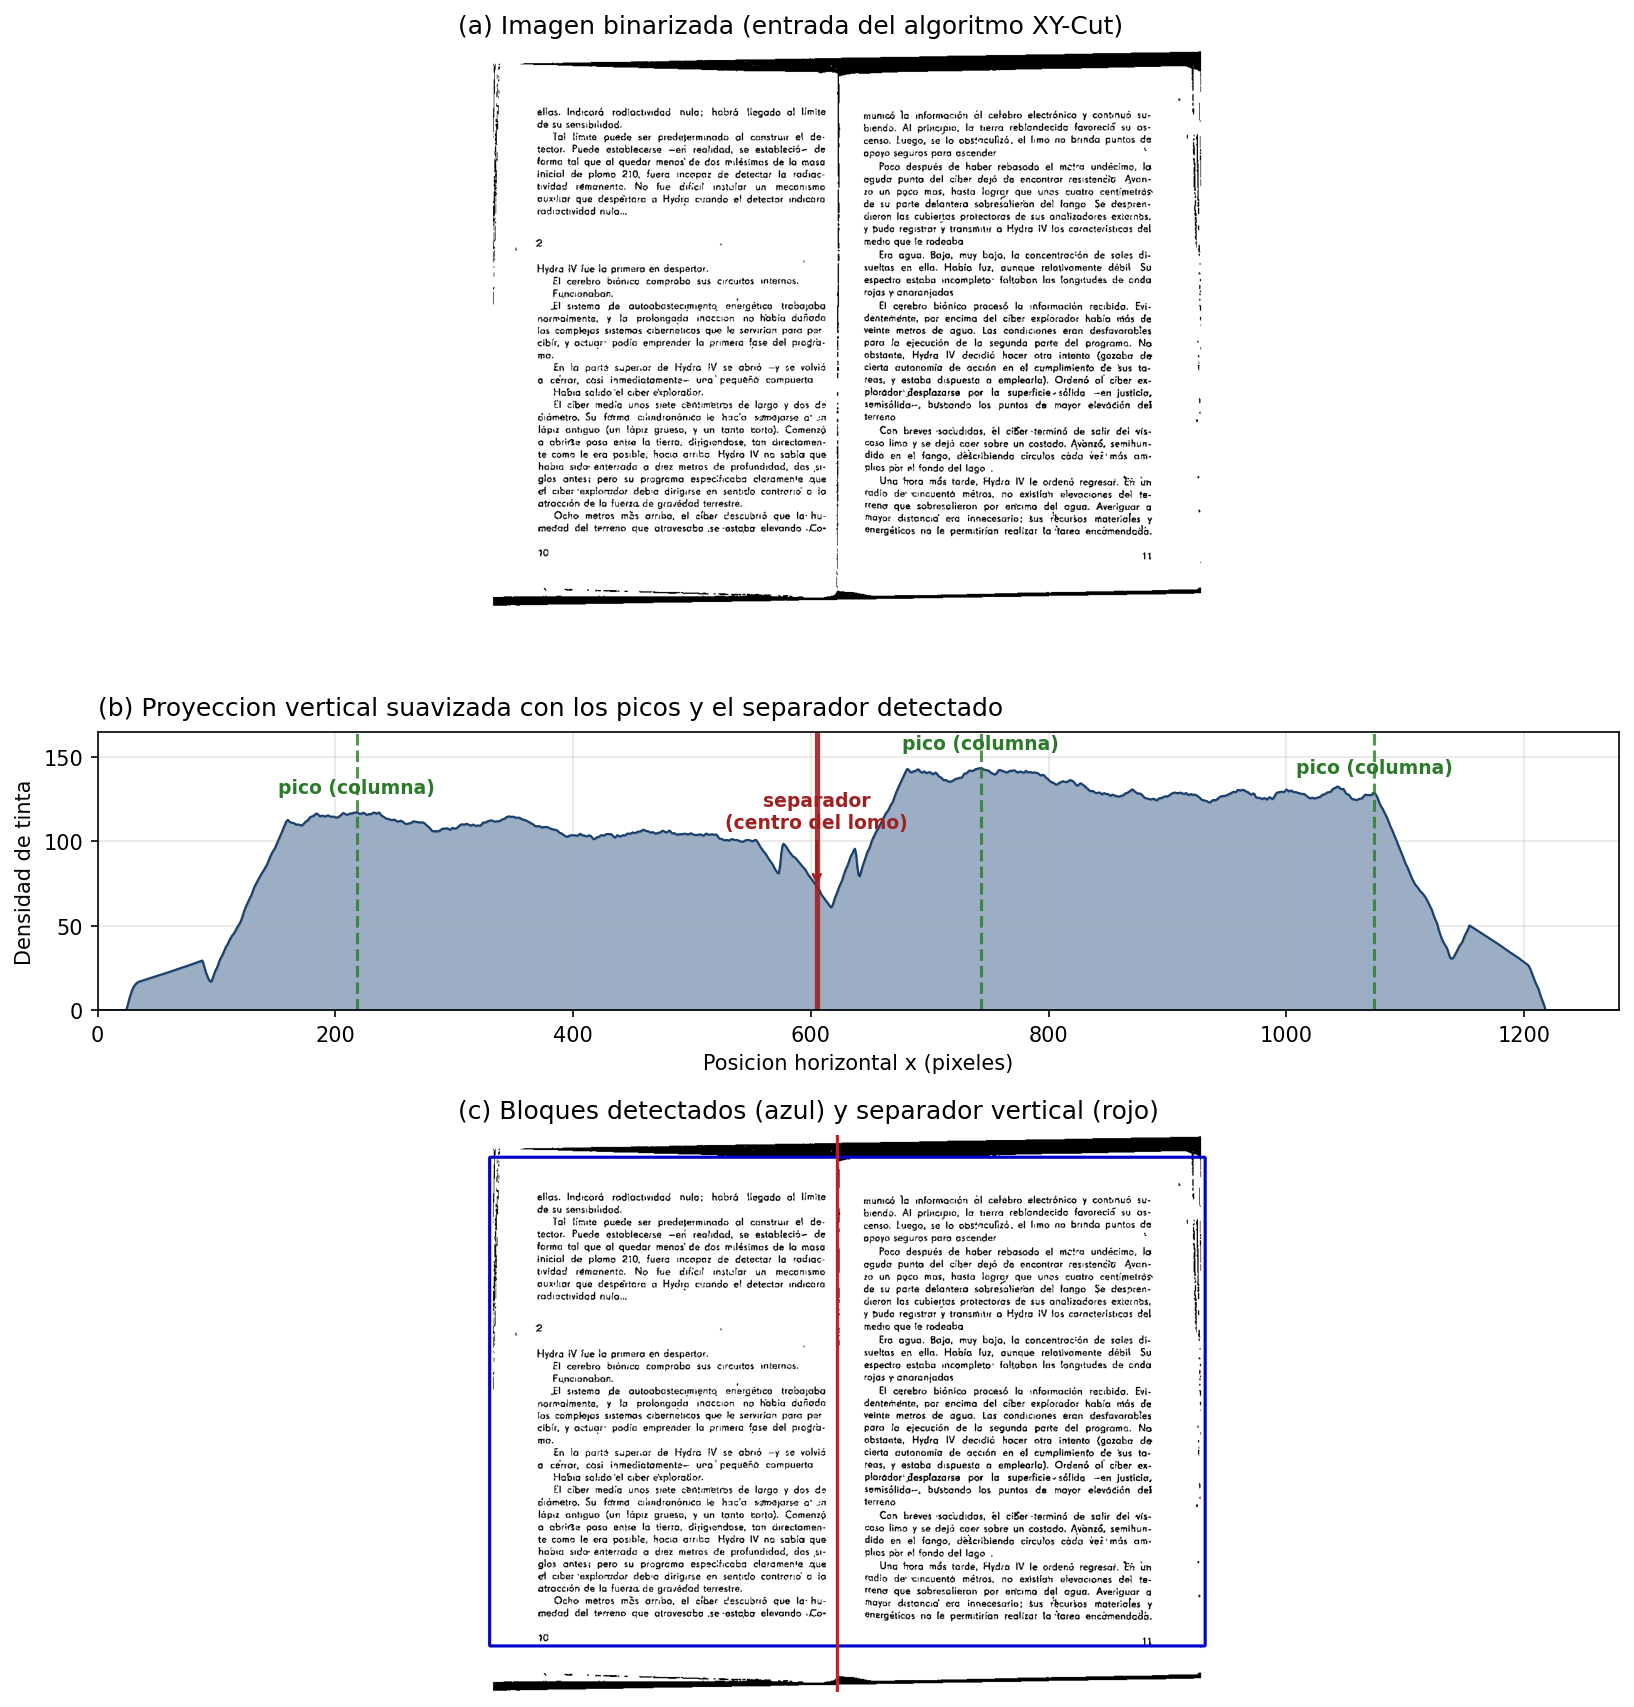
\includegraphics[width=0.95\textwidth]{Graphics/xy_cut_proceso.png}
	\caption{Detección de bloques sobre un pliego digitalizado mediante el algoritmo XY-Cut. El panel (a) muestra la imagen binarizada que sirve de entrada al algoritmo. El panel (b) muestra la proyección vertical tras el suavizado, los picos que corresponden a cada columna y el separador que el método coloca en el centro del hueco entre páginas. El panel (c) muestra los bloques detectados sobre la imagen original.}
	\label{fig:xy-cut}
\end{figure}

El candidato a separador se acepta solo si la profundidad del valle supera el 28\,\% de la altura del pico menor de los dos, si el ancho del hueco supera un umbral mínimo, y si la posición del separador queda dentro del rango central del 15 al 85\,\% del ancho de la imagen. La triple condición rechaza separadores que aparecerían en imágenes con una sola columna pero con variaciones locales de densidad. El algoritmo admite hasta cuatro columnas por banda; cuando el número de candidatos excede el límite, el sistema conserva los separadores con la profundidad de valle mayor.

Antes de aplicar el algoritmo, una máscara cubre las franjas laterales que corresponden a la encuadernación. La medida evita que el moteado oscuro del borde del escáner aparezca como contenido de texto y desplace los cortes hacia el interior de la página. Tras la segmentación, el sistema fusiona en un único bloque los bloques resultantes que quedan a una distancia inferior a un umbral, lo que evita la sobresegmentación de columnas que el algoritmo dividió en exceso por la presencia de espacios verticales puntuales dentro del texto.

\subsection{Segmentación de líneas dentro de cada bloque}

Dentro de cada bloque, el \textit{pipeline} segmenta las líneas mediante proyección horizontal con dilatación morfológica previa. La dilatación horizontal une las palabras de una misma línea para que la proyección presente un máximo continuo a lo largo del renglón. La dilatación vertical, mucho más pequeña, conecta los acentos de las mayúsculas con el cuerpo de la letra correspondiente, lo que evita que los acentos generen picos secundarios en la proyección.

Un filtro uniforme suaviza la proyección horizontal resultante. El método umbraliza la proyección suavizada con un valor que el método de Otsu~\cite{otsu1979threshold} produce sobre el perfil unidimensional. El umbral final queda acotado al~25\,\% del pico máximo de la proyección, valor que el trabajo calibró para que las líneas cortas de final de párrafo, cuya proyección puede ser entre tres y cinco veces menor que la de líneas completas, queden por encima del umbral.

La salida de la segmentación es una lista de cajas delimitadoras, con las coordenadas verticales y horizontales de cada esquina del segmento en la imagen original. El algoritmo expande ligeramente cada caja hacia los píxeles de tinta adyacentes que probablemente quedaran fuera del corte estricto por proyección. La línea final corresponde al recorte de la imagen original en la región que delimita la caja expandida.

% -----------------------------------------------------------------------------
\section{Normalización de líneas para inferencia}
\label{sec:normalizacion-lineas}

Las líneas que salen del paso de segmentación presentan dimensiones heterogéneas. La altura varía con el tamaño tipográfico, la presencia de descendentes y ascendentes y el ajuste de la caja delimitadora. El ancho varía con la longitud del texto. El modelo de reconocimiento exige, sin embargo, una altura fija para sus entradas, según argumenta el capítulo~\ref{chap:modelo}. La sección describe el procedimiento de normalización que produce las líneas con el formato que el modelo espera.

El procedimiento se descompone en tres operaciones secuenciales. La primera es el recorte vertical. El sistema localiza las filas con presencia de tinta y recorta la línea a la región vertical mínima que las contiene, con un margen de seguridad dinámico igual al 10\,\% de la altura del texto. El margen evita que descendentes y ascendentes queden cortados por un ajuste demasiado ceñido.

La segunda operación es el redimensionado a una altura fija de~64 píxeles, manteniendo la proporción original entre alto y ancho. El trabajo eligió la altura fija de~64 píxeles por dos razones. La primera es la compatibilidad con la arquitectura convolucional del modelo: el codificador aplica cuatro reducciones de la altura por un factor de dos, lo que requiere que la altura de entrada sea divisible por~16. La segunda es el equilibrio entre detalle visual preservado y coste computacional. Alturas menores comprimen los caracteres hasta perder rasgos finos. Alturas mayores aumentan el coste de cómputo sin mejora apreciable en exactitud para los cuerpos tipográficos habituales en documentos impresos. El ancho resultante es variable y queda determinado por la proporción de la línea original.

La tercera operación es la conversión de la imagen a tensor en coma flotante con valores normalizados al intervalo $[0, 1]$. La operación produce el formato exacto que el modelo CRNN+CTC~\cite{shi2016crnn,graves2006ctc} consume como entrada durante la inferencia.

La contribución cuantitativa de cada etapa del \textit{pipeline} sobre el rendimiento del modelo final no se evalúa mediante un estudio de ablación específico en este trabajo. La razón es metodológica: cada etapa cumple una función no opcional dentro del flujo --la binarización produce la representación que el extractor convolucional del modelo espera, la corrección de inclinación habilita la proyección horizontal que la segmentación de líneas necesita, la segmentación produce las líneas que el modelo procesa, y la normalización ajusta la altura que la arquitectura impone--, por lo que su eliminación produciría una caída catastrófica de la métrica que un estudio de ablación constataría sin aportar información cuantitativa interpretable. La validación de cada técnica descansa, por tanto, en la evidencia empírica que la literatura previa aporta sobre documentos impresos: Otsu~\cite{otsu1979threshold} y Sauvola~\cite{sauvola2000binarization} sustentan la binarización adaptativa con selección entre umbral global y umbral local según el criterio de uniformidad de fondo, y Duda y Hart~\cite{duda1972hough} sustentan la transformada que detecta la orientación dominante para la corrección de inclinación. Un estudio de ablación que cuantifique la contribución marginal de cada parámetro de cada etapa sobre el \textit{corpus} propio constituye una línea natural de extensión del trabajo.

% -----------------------------------------------------------------------------
% Transición al capítulo 4
% -----------------------------------------------------------------------------

Con el \textit{pipeline} de preprocesamiento que el capítulo describe, queda cerrado el camino que transforma una página digitalizada en una lista de líneas con el formato que el modelo de reconocimiento espera. El capítulo siguiente aborda la tercera contribución técnica del trabajo: el diseño, el entrenamiento y la evaluación del modelo CRNN+CTC que produce la transcripción de cada línea normalizada.
